\subsection{Anillos de polinomios}

\subsubsection{Propiedades generales}

\begin{definition}[Polinomios con coeficientes en un anillo conmutativo]
	Dado un anillo commutativo A y un símbolo X no usado para representar elementos de A. 
	
	Un polinomio es una función de coeficientes $f: \mathbb{N} \to A$ de soporte finito: $$\exists n \in \mathbb{N}. \forall m > n. f(m) = 0$$ es decir, toma valor no nulo en un subconjunto finito de $\mathbb{N}$. 
	
	Se denomina coeficiente líder al mayor $n$ tal que $f(n) \neq 0$. 
	
	En el conjunto de todos los polinomios sobre $A$ definimos dos operaciones:
	
	\begin{itemize}
		\item Suma de polinomios: $(f,g) \mapsto f+g$ tal que $\forall n \in \mathbb{N}.(f+g)(n) = f(n) +g(n)$
		\item Producto de polinomios: $(f,g) \mapsto f \cdot g$ tal que $ \forall n \in \mathbb{N}.(f \cdot g)(n) = \sum_{i+j = n} f(i) g(j)$
	\end{itemize}
\end{definition}

\begin{proposition}[Estructura de anillo conmutativo de los polinomios]
	El conjunto $A[X]$ de los polinomios con coeficientes en $A$ es un anillo conmutativo. 
\end{proposition}
\begin{proof}
	Claramente, las operaciones son internas:
	
	Dados $f,g \in A[X]$ tenemos que $\exists. n_f,n_g$ tales que $\forall n > n_f. f(n) = 0 \land \forall n > n_g. g(n) = 0$. 
	
	Tomando $n_+ = max\{n_f,n_g\}$ tenemos que $\forall n > n_+. (f+g)(n) = f(n)+g(n) = 0$. Por tanto, $f+g \in A[X]$. 
	Tomando $n_\cdot = n_f + n_g$ tenemos que $\forall n > n_\cdot. (f \cdot g)(n) = \sum_{i+j = n} f(i)g(j)$ dado que $i,j \in \mathbb{N} \land i+j > n_f + n_g$ necesariamente $i > n_f \lor j > n_g$ en cuyo caso todos los términos $f(i)g(j)$ son cero. Por tanto, $f \cdot g \in A[X]$. 
	
	Las propiedades de asociatividad para la suma y la commutividad son fáciles de ver. Veamos como se demuestra la asociatividad para el producto:
	
	$(f(gh))(n) = \sum_{i+m = n} f(i)(gh)(m) = \sum_{i+m = n} f(i) (\sum_{j+k = m} g(j)h(k)) = \sum_{i+m = n \land j+k = m} f(i)g(j)h(k) = \sum_{i+j+k = m} f(i)g(j)h(k)$. Donde la última igualdad se verifica por la propiedad de distributividad generalizada. 
	
	El elemento neutro para la suma es el polinomio $0: \mathbb{N} \to A$ tal que $\forall n \in \mathbb{N}. 0(n) = 0$. 
	
	El elemento neutro para el producto es el polinomio $1:\mathbb{N} \to A$ tal que $1(0) = 1 \land \forall n > 0. 1(n) = 0$. En efecto, $(f\cdot 1)(n) = \sum_{i+j = n} f(i)1(j) = f(n)1(0) = f(n)$. 
	
	El elemento opuesto de un polinomio $f$ es el polinomio $-f: \mathbb{N} \to A$ tal que $\forall n. (-f)(n) = -f(n)$. 
	
	Se verifica la distributividad de la suma respecto del producto:
	
	$f \cdot (g+h)(n) = \sum_{i+j = n} f(i) (g+h)(j) = \sum_{i+j = n} (f(i)g(j) + f(i)h(j)) = \sum_{i+j = n} f(i)g(j) + \sum_{i+j = n} f(i)h(j) = (f\cdot g + f \cdot h)(n)$.  
\end{proof}

\begin{definition}[Polinomios destacados]
	Consideremos un anillo de polinomios $A[X]$. 
	
	Un polinomio $f \in A[X]$ es constante si $\forall n > 0. f(n) = 0$. Si $f(0) = a$ lo denotamos por $a$. 
	
	La potencia k-ésima de x es el polinomio$f: \mathbb{N} \to A$ tal que $f(k) = 1 \land \forall n \neq k. f(n) = 0$. Lo denotaremos por $x^k$.  
	
	Un polinomio con un único coeficiente no nulo se llama monomio. 
\end{definition}

\begin{definition}[Grado de un polinomio]
Dado $f \neq 0$ un polinomio no nulo. El grado de f es un número natural $n$ tal que $p(n) \neq 0 \land \forall m > n. f(m) = 0$. Por convención al polinomio nulo se le asigna grado $-\infty$. 

El símbolo $-\infty \notin \mathbb{N}$ se lee \textit{ menos infinito } y se opera con él mediante las siguientes reglas formales:

\begin{itemize}
\item $\forall n \in \mathbb{N}.-\infty < n$
\item $-\infty + n = -\infty = n + (-\infty)$
\item $-\infty  n = -\infty = n (-\infty)$
\item $-\infty + -\infty = -\infty$
\end{itemize} 
\end{definition}

\begin{proposition}[Anillo de coeficientes como subanillo del anillo de polinomios]
	Si identificamos $A$ con el conjunto de los polinomios constantes, entonces $A$ es un subanillo de $A[X]$. 
\end{proposition}
\begin{proof}
	En efecto, las operaciones suma y producto de $A[X]$ son cerradas para el conjunto de los polinomios constantes. También $1,-1$ son polinomios constantes. 
\end{proof}

\begin{lemma}[Identificación del monomio de grado $k$ con coeficiente $a$]
	$\forall k \ge 0, a \in A \setminus \{0\}$, $a \cdot x^k$ es el monomio de grado k con coeficiente a en grado k. 
\end{lemma}
\begin{proof}
	La demostración se hace por inducción sobre k. Para $k = 0$, se verifica que $ax^0 = a$. 
	
	Suponiendo que es cierto para $k$ se compruebra que es cierto para $ax^{k+1}$. En efecto, $(ax^{k+1})(n) = ((ax^k)x)(n) = \sum_{i+j = n} (ax^k)(i)x(j) = (ax^k)(n-1)$ y por hipótesis de inducción sabemos que este polinomio vale $a$ si $k = n-1$ y cero en otro caso, luego el polinomio original vale $a$ en k+1 y cero en otro caso. 
\end{proof}

\begin{definition}[Notación de un polinomio como suma de monomios]
	Dado $f \in A[X]$ tal qque $\forall n \in \mathbb{N}. f(n) = a_n$. 
	
	Representamos este polinomio mediante la expresión $\sum_{n \ge 0} a_nx^n$. 
\end{definition}

Podemos comprobar que ambas expresiones representan el mismo polinomio: $$\sum_{n \ge 0} a_n x^m)(m) = \sum_{n \ge 0} (a_n x^n)(m) = (a_mx^m)(m) = a_m = f(n)$$

Usando esta notación multiplicaríamos del siguiente modo: $$(\sum_{n \ge 0} a_n x^n)(\sum_{n \ge 0} b_n x^n) = \sum_{n,m \ge 0} a_n b_m x^{n+m} = \sum_{n \ge 0} (\sum_{n+m = k} a_nb_m) x^k$$ 

\begin{example}
	Consideramos $f = 2+5x+4x^2, g = 1+3x \in \mathbb{Z}_6[X]$, claramente $f+g=3+2x+4x^2, -g = 5+3x,f\cdot g = 2 + 5x + x^2$. Nótese que aquí $grado(f \cdot g) \neq grado(f) + grado(g)$. Esta fórmula sólo será cierta cuando el anillo original sea un dominio de integridad. 
\end{example}

El siguiente teorema nos dice que para cada $u$ el homomorfismo con ciertas propiedades $f_u$ es universal para la clase de homomorfismos que tienen como dominio $A$, esto es, cualquier homomorfismo sobre $A$ factoriza por su anillo de polinomios. 

\begin{theorem}[Propiedad universal de los anillos de polinomios]
	Dados $A,B$ dos anillos conmutativos y un homomorfismo $f: A \to B$. Dado $u \in B$ existe un único homomorfismo de anillos $f_u: A[X] \to B$ tal que $\forall a \in A:f_u(\lambda(a)) = f(a)$ y $f_u(x) = u$. Donde $\lambda$ es la inclusión de $A$ en $A[X]$. 
	
	\begin{tikzcd}
		A \arrow{r}{\lambda} \arrow{dr}{f} &
		A[X] \arrow[dashed]{d}{f_u} \\
		& B \ni u
	\end{tikzcd}
	
	$f_u$ está dado por $f_u(\sum_{i \ge 0} a_iX^i) = \sum_{i \ge 0} f(a_i)u^i$. 
\end{theorem}
\begin{proof}
	Dado $p = \sum_{n \ge 0} a_n x^n \in A[X]$, defino $f_u(p) = \sum_{n \ge 0} f(a_n)u^n$.
	
	Claramente, $f_u$ satisface las propiedades requeridas y su codominio es $B$. Además es un homomorfismo. En efecto, $f_u(1) = 1$ y $$f_u(pq) = f\Big(\sum_{n \ge 0} \Big(\sum_{i+j = n} a_ib_j\Big)u^n\Big) = \sum_{n \ge 0} f\Big(\sum_{i+j = n} a_ib_j\Big)u^n = \sum_{n \ge 0} \Big(\sum_{i+j = n} f(a_i)f(b_j)\Big)u^n$$ donde se ha utilizado la definición de $f_u$ y que $f$ es un homomorfismo y por otro lado: $$f_u(p)f_u(q) = \Big(\sum_{n \ge 0} f(a_n) u^n\Big)\Big(\sum_{n \ge 0} f(b_n) u^n\Big) = \sum_{i,j \ge 0} f(a_i)u^if(b_j)u^j = \sum_{i,j \ge 0} f(a_i)f(b_j)u^{i+j} = \sum_{n \ge 0} \Big(\sum_{i+j = n} f(a_i)f(b_j)\Big)u^n$$ donde se ha utilizado la asociatividad generalizada y el hecho de que el anillo es conmutativo. Claramente, ambas expresiones son iguales. También es fácil demostrar que $f_u(p+q) = f_u(p) + f_u(q)$. 
	
	Finalmente, $f_u$ es el único homomorfismo que verifica las propiedades requiridas. En efecto, si $\phi:A[X] \to B$ verifica $\forall a \in A. \phi(\lambda(a)) = f(a) \land \phi(x) = u$ entonces $$\phi\Big(\sum_{n \ge 0} a_n x^n\Big) = \sum_{n \ge 0} \phi(a_n x^n) = \sum_{n \ge 0} \phi(a_n) \phi(x)^n = \sum_{n \ge 0} f(a_n) u^n = f_u\Big(\sum_{n \ge 0} a_n x^n\Big)$$
\end{proof}

\begin{definition}[Anillo de polinomios en dos indeterminadas]
	Dado un anillo conmutativo $A$ e $Y$ un símbolo que no denota a ningún elemento de $A[X]$. Definimos el anillo de polinomios en dos indeterminadas como $A[X,Y] = A[X][Y] = A[Y][X]$ donde el producto se realiza como $$(\sum_{i,j \ge 0} a_{ij}x^iy^j)(\sum_{k,l \ge 0} b_{kl}x^ky^l) = \sum_{i,j,k,l \ge 0} a_{ij}b_{kl} x^{i+k}y^{j+l} = \sum_{m,n \ge 0} (\sum_{i+k = m \land j+l = n} a_{ij}b_{kl}) x^m y^n$$ donde hemos utilizado la propiedad distributiva generalizada y la propiedad commutativa del producto. 
\end{definition}

\begin{proposition}[Buena definición del anillo de polinomios en dos indeterminadas]
	La anterior, es una buena definición.
\end{proposition}
\begin{proof}
	Dado $f \in A[X][Y]$, $f$ es de la forma $\sum_{j \ge 0} f_j(x) y^j$ con $f_j(x) \in A[X]$, si escribimos $f_j(x) = \sum_{i \ge 0} a_{ij} x^i$ nos queda para $f$: $$f = \sum_{j \ge 0} (\sum_{i \ge 0} a_{ij} x^i) \cdot y^j = \sum_{i,j \ge 0} a_{ij} x^i y^j = \sum_{i,j \ge 0} a_{ij} y^j x^i = \sum_{i \ge 0} (\sum_{j \ge 0} a_{ij} y^j)x^i = \sum_{i \ge 0} g_j(y) x^i \in A[Y][X]$$ donde hemos utilizado la propiedad distributiva generalizada con uno de los factores de longitud uno repetidas veces. Esto demuestra que $A[X][Y] = A[Y][X]$ de donde la definición anterior es buena. 
\end{proof}

\begin{definition}[Anillos de polinomios multivariados]
	Definimos inductivamente $A[X_1,\cdots,X_r]$:
	
	Para $r = 1$ no hay nada que definir. Supuesto definido para $r$, $A[X_1, \cdots, X_{r+1}] = A[X_1, \cdots, X_r][X_{r+1}]$.
	
	Los elementos de $A[X_1,\cdots,X_r]$ se expresan como $\sum_{i_1,\cdots,i_r} a_{i_1}\cdots a_{i_r} x_1^{i_1} \cdots x_r^{i_r}$.
\end{definition}

\begin{theorem}[Propiedad universal de los anillos de polinomios multivariados]
	Dados $A,B$ dos anillos conmutativos y un homomorfismo $f: A \to B$. Dado $u \in B^k$ existe un único homomorfismo de anillos $f_u: A[X_1,\cdots,X_r] \to B$ tal que $\forall a \in A:f_u(\lambda(a)) = f(a)$ y $f_u(x_i) = u_i$. Donde $\lambda$ es la inclusión de $A$ en $A[X_1,\cdots,X_r]$. 
	
	\begin{tikzcd}
			A \arrow{r}{\lambda} \arrow[swap]{drr}{f} &
			A[X_1,\ldots,X_{r-1}] \arrow{dr}{g} \arrow{r}{\lambda} &
			A[X_1,\ldots,X_{r-1}][X_r] \arrow{d}{h} \\
			& & B 
	\end{tikzcd}
\end{theorem}
\begin{proof}
	Procedemos por inducción sobre $n$. El caso $n = 1$ está demostrado. Supongamos que la propiedad es cierta para $r-1$ y veámoslo para $r$. Dado $u \in B^k$ por hipótesis de inducción existe un único homomorfismo de anillos $g:A[A_1,\cdots,X_{r-1}] \to B$ tal que $\forall a \in A. g(\lambda(a)) = f(a) \land g(x_i) = b_i$ con $1 \le i \le r-1$. Luego aplicamos el caso $n = 1$ con $A = A[X_1,\cdots,X_{r-1}]$ y obtenemos un único homomorfismo $h:A[X_1,\cdots,X_{r-1}][X_r] \to B$ tal que $\forall p \in A[A_1, \cdots,X_{r-1}]. h(\lambda(p)) = g(p) \land g(x_r) = b_r$. Por las características de $g$ está claro que $h$ es un homomorfismo con las propiedades requeridas por el teorema. 
\end{proof}

\subsubsection{Raíces, derivada y fórmula de Taylor}

\begin{definition}[Morfismo de evaluación]
Un caso particular de la propiedad universal de los anillos de polinomios univariados, se da cuando $A$ es subanillo de $B$ y $f$ es la inclusión. En este caso, $f_u$ se denota por $E_u$ y se llama morfismo de evaluación en u. Claramente, $E_u(\sum_{n \ge 0} a_n x^n) = \sum_{n \ge 0} a_n u^n \equiv f(u)$. Este homomorfismo permite el cálculo del valor de un  polinomio en cualquier punto.
\end{definition}

\begin{definition}[Raíz de un polinomio]
$\alpha$ es raíz de $f \in A[X]$ si $f(\alpha) = 0$. 
\end{definition}

Contar con el algoritmo de la pseudo-división nos permite hablar de raíces en polinomios cuyos coeficientes no forman parte de un cuerpo. 

\begin{proposition}[Caracterización de las raíces de un polinomio]
$\alpha$ es raíz de $f \in A[X] \iff (X-\alpha) | f$
\end{proposition}
\begin{proof}
$\Rightarrow)$ Pseudo-dividimos $f$ entre $X-\alpha$ y obtendríamos $f = (X-\alpha)q + r$ con $r = 0 \lor gr(r) < gr(X-\alpha) = 1 \implies gr(r) = 0$. Evaluando en $\alpha$ obtendríamos que $f(\alpha) = r$. Por tanto, si $\alpha$ es raíz de $f$, $r = 0$ y por tanto, $X-\alpha|f$. 

$\Leftarrow)$ Si $(X-\alpha)|f$ entonces $f = (X-\alpha)g$ con $g \in A[X]$. Evaluando en $\alpha$, $f(\alpha) = 0$ y por tanto, $\alpha$ es raíz de $f$. 
\end{proof}

\begin{definition}[Derivada de un polinomio]
Sea $A$ un anillo cualquier y $f = \sum_{i \ge 0} a_iX^i \in A[X]$, la derivada de $f$ es $f' = \sum_{i \ge 1} ia_i^{i-1}$
\end{definition}

\begin{proposition}[Primeras propiedades]
Sean $f,g \in A[X]$ y $a \in A$. 

\begin{enumerate}
\item $(af)' = af'$
\item $(f+g)' = f'+g'$
\item $(fg)' = f'g + fg'$
\end{enumerate}
\end{proposition}

\begin{definition}[Raíz múltiple]
Una raíz $\alpha \in A$ de $f \in A[X]$ es raíz múltiple de $f$ si $(X-\alpha)^2 | f$. 
\end{definition}

\begin{proposition}[Caracterización de raíces múltiples]
$\alpha \in A$ es una raíz múltiple de $f$ $\iff f(\alpha) = f'(\alpha) = 0$.
\end{proposition}
\begin{proof}
$\Rightarrow)$ Si $\alpha$ es raíz múltiple entonces $f = (X-\alpha)^2g$ de donde claramente $f(\alpha) = 0$ y además $f' = 2(X-\alpha)g + (X-\alpha)^2g' = (X-\alpha)(2g + (X-\alpha)g')$. En consecuencia, $f'(\alpha) = 0$. 

$\Leftarrow)$ Si $f(\alpha) = 0$ entonces $\alpha$ es raíz de $f$ y por tanto, $(X-\alpha)$ divide a $f$. Por tanto, $f = (X-\alpha)h \implies f' = h+(X-\alpha)h'$ y como $f'(\alpha) = 0$ entonces también $h(\alpha) = 0$ y por tanto, $(X-\alpha)|h \implies h = (X-\alpha)K \implies f = (X-\alpha)^2K$.
\end{proof}

\begin{definition}[Desarrollo de Taylor]
Sea $K$ un cuerpo y $\alpha \in K$. 

En la propiedad universal del anillo polinomios consideramos el homomorfismo inclusión $i:K \to K[X]$ y existirá un único homomorfismo $K[X] \to K[X]$ tal que $X \mapsto X-\alpha$. Es claro que este homomorfismo es $T(f(X)) = f(X-\alpha)$. 

En particular, si restringimos $T$ a $\mathbb{P}_n(K)$, $T$ es una aplicación $K$-isomorfismo de espacios vectoriales. En particular, $T(\{1,X,\ldots,X^n\}) = \{1,X-\alpha,\ldots,(X-\alpha)^n \}$ es una base. 

Dado un polinomio $f \in K[X]$, $f = \sum \alpha_i (X-\alpha)^i$ y se comprueba por inducción que $n!\alpha_n = f^{n)}(\alpha)$. Si la característica del cuerpo es no nula algún $n!$ podría ser cero y si sustituimos directamente estaríamos dividiendo por cero. Por tanto, si asumimos que la característica no es cero entonces $f = f(\alpha) + \ldots + \frac{1}{n!}f^{n)}(\alpha)(X-\alpha)^n$. 
\end{definition}

\begin{definition}[Raíces simples y múltiples]
Sea $\alpha$ una raíz múltiple de $f \in K[X]$.

$\alpha$ tiene multiplicidad $m \ge 2$ si $(X-\alpha)^m|f$ pero $(X-\alpha)^{m+1} \nmid f$. 

$\alpha$ es raíz simple si no es múltiple. 
\end{definition}

\begin{proposition}[Caracterización de la multiplicidad]
Sea $K$ un cuerpo de característica $0$ y $\alpha \in K$. 

Dado $f \in K[X]$, $\alpha$ es raíz múltiple de $f$ de multiplicidad $m \iff f(\alpha) = f'(\alpha) = \ldots = f^{m-1)}(\alpha) = 0$ pero $f^{m)}(\alpha) \neq 0$. 
\end{proposition}
\begin{proof}
$\Rightarrow)$ Supongamos que la multiplicidad de $\alpha$ como raíz es $m$. Entonces, $f(X) = (X-\alpha)^mh(X)$ con $h(\alpha) \neq 0$. Entonces: $$f'(X) = m(X-\alpha)^{m-1}h(X)+(X-\alpha)^mh'(X)$$ y, evaluando en $\alpha$, tendríamos que $f'(\alpha) = 0$. Se procede por inducción para demostrar el resto del enunciado. 

$\Leftarrow)$ Se utiliza el desarrollo de Taylor. 
\end{proof}

\subsection{Anillos de enteros cuadráticos}

\begin{definition}[Enteros cuadráticos]
Para cada $n \in \mathbb{Z}$ que no sea cuadrado perfecto, se define el conjunto de los enteros cuadráticos de radicando n como $\mathbb{Z}[\sqrt{n}] = \{a+b\sqrt{n}:a,b \in \mathbb{Z}\}$.

A este conjunto se le dota de estructura de anillo mediante las operaciones:

\begin{itemize}
\item Suma: $(a+b\sqrt{n})+(c+d\sqrt{n}) = (a+c) + (b+d)\sqrt{n}$
\item Producto: $(a+b\sqrt{n}) \cdot (c+d\sqrt{n}) = (ac+bdn)+(ad+bc)\sqrt{n}$
\end{itemize}

Dado un entero cuadrático $x = a + b \sqrt{n} \in \mathbb{Z}[\sqrt{n}]$ definimos su conjugado $\overline{x} = a - b \sqrt{n}$ y su norma como $N(x) = x \overline{x} = a^2-nb^2$. 
\end{definition}

\begin{proposition}[Propiedades generales]
1. $\mathbb{Z} \subseteq \mathbb{Z}[\sqrt{n}] \land \mathbb{Z} = \mathbb{Z}[\sqrt{n}] \iff n$ es un cuadrado perfecto. \\
2. $\mathbb{Z}[\sqrt{n}]$ es un subanillo de $\mathbb{C}$ y si $n > 0$ entonces $\mathbb{Z}[\sqrt{n}]$ es un subanillo de $\mathbb{R}$. \\
3. $-:\mathbb{Z}[\sqrt{n}] \to \mathbb{Z}[\sqrt{n}]$ es un homomorfismo de anillos idempotente.\\
4. $N:\mathbb{Z}[\sqrt{n}] \to \mathbb{Z}$ es un homomorfismo de monoides conmutativos.\\
5. $U(\mathbb{Z}[\sqrt{n}]) = \{x: N(x) \in \{1, -1\}\}$. 
\end{proposition}
\begin{proof}
1. Trivial.

2. Basta comprobar que la suma y el producto son cerradas en $\mathbb{Z}[\sqrt{n}]$ y se corresponden con las operaciones de los complejos. También se verifica que $1,-1 \in \mathbb{Z}[\sqrt{n}]$ de donde se tiene que es un subanillo de los complejos. La otra propiedad es entonces trivial. 

3. Si $x = (a,b) \land y = (c,d)$ entonces:

\begin{itemize}
\item $\overline{x+y} = \overline{(a+c,b+d)} = (a+c,-b-d) = (a,-b) + (c,-d) = \overline{x} + \overline{y}$.
\item $\overline{xy} = (ac+bdn,-ad-bc) = (a,-b) \cdot (c,-d) = \overline{x} \cdot \overline{y}$.
\item $\overline{1} = 1$. 
\end{itemize} 

4. Por las propiedades de la conjugación:

\begin{itemize}
\item $N(xy) = (xy)(\overline{xy}) = xy \cdot \overline{x} \cdot \overline{y} = x \overline{x}\overline{y} = N(x)N(y)$
\item $N(1) = 1^2-0n = 1$
\end{itemize}

5. $\subseteq)$ Como $N$ es un homomorfismo multiplicativo, preserva las unidades y por tanto, si $x \in U(\mathbb{Z}[\sqrt{n}]) \implies x \in U(\mathbb{Z}) = \{1,-1\}$.

$\supseteq)$ Observemos que $N(x) = x\overline{x}$. Si $N(x) = 1$ entonces $x^{-1} = \overline{x}$ y si $N(x) = -1$ entonces  $x^{-1} = - \overline{x}$. Luego en cualquier caso tenemos una unidad del anillo.  
\end{proof}

\begin{example}[Unidades para distintos radicandos]
Veamos cuál es la situación según el signo de $n$. 

\begin{enumerate}
\item El anillo de los enteros de Gauss es $\mathbb{Z}[i] = \{a+bi:a,b \in \mathbb{Z}\}$. Está claro que en este anillo $N(a+bi) = a^2 + b^2$ y las soluciones de $N(a+bi) = 1 \lor N(a+bi) = -1$ son las parejas $(a,b)$ de la forma $(0,1),(0,-1),(1,0),(-1,0)$. Por tanto, $U(\mathbb{Z}[i]) = \{1,-1,i,-i\}$. 

\begin{figure}[H]
\centering
\makebox[\textwidth][c]{
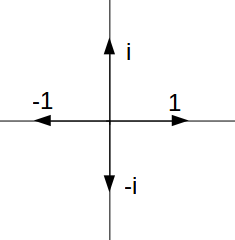
\includegraphics[scale=0.5]{./images/roots.png}
}
\end{figure}

\item En general si $n < 0$ entonces la ecuación $N(x) = a^2 - nb^2 = a^2 + (-n)b^2 = -1$ no tiene solución y debemos considerar sólo las soluciones de $N(x) = a^2 - nb^2 = a^2 + (-n)b^2 = 1$. Para $n = 1$, tenemos el caso anterior y si $n > 1$ entonces es claro que sólo hay dos soluciones que son $1,-1$. 

\item El anillo de los enteros cuadráticos de radicando 2 es $\mathbb{Z}[\sqrt{2}] = \{a+b\sqrt{2}:a,b \in \mathbb{Z}\}$. Este anillo tiene como unidades todas las soluciones $(a,b)$ de las ecuaciones $a^2-2b^2 = 1 \lor a^2-2b^2 = -1$. Obsérvese que como $N(1+ \sqrt{2}) = -1$ entonces $N((1+\sqrt{2})^k) = (-1)^k$ y por tanto todo $(1+\sqrt{2})^k$ son unidades del anillo. Se puede demostrar que todas las unidades del anillo son de esta forma. 

\item En general, el fenómeno del apartado anterior se da para $n > 0$ y al elemento base de las potencias se le llama solución fundamental. 
\end{enumerate}
\end{example}

